\newpage

\section{Data Understanding}

\subsection{Data Overview}

The dataset used in this project contains financial transaction records, including both legitimate and fraudulent activities.

\textbf{General Information}
\begin{itemize}
    \item Number of records: 1,296,675
    \item Number of features: 23
    \item Target variable: is\_fraud
\end{itemize}

\textbf{Fraud Analysis}
\begin{itemize}
    \item Fraud count: 7,506
    \item Fraud ratio: 0.005789 (0.58\%)
\end{itemize}

This indicates a severe class imbalance problem, where fraudulent transactions are extremely rare compared to normal transactions.

\subsection{Feature Description}

The dataset consists of multiple types of features, which can be grouped as follows:

\subsubsection{Identification Features}
\begin{itemize}
    \item stt: Transaction index
    \item cc\_num: Customer credit card number
    \item trans\_num: Unique transaction identifier
\end{itemize}

\textbf{Observation:} These features serve as identifiers and do not provide meaningful predictive information for fraud detection.

\subsubsection{Time Features}
\begin{itemize}
    \item trans\_date\_trans\_time: Timestamp of the transaction
    \item unix\_time: Transaction time in Unix timestamp format
\end{itemize}

\textbf{Applications:}
\begin{itemize}
    \item Extract temporal features such as:
    \begin{itemize}
        \item hour of the transaction
        \item day of the week
    \end{itemize}
    \item Detect abnormal transaction timing patterns
\end{itemize}

\subsubsection{Transaction Features}
\begin{itemize}
    \item amt: Transaction amount
    \item category: Type of transaction (e.g., shopping, dining, entertainment)
    \item merchant: Merchant name
\end{itemize}

\textbf{Observation:}
\begin{itemize}
    \item The transaction amount (amt) is a critical feature
    \item The category helps identify spending behavior patterns
\end{itemize}

\subsubsection{Customer Information}
\begin{itemize}
    \item first, last: Customer name
    \item gender: Gender of the customer
    \item dob: Date of birth
    \item job: Occupation
\end{itemize}

\textbf{Applications:}
\begin{itemize}
    \item Derive age from date of birth
    \item Analyze demographic-based transaction behavior
\end{itemize}

\subsubsection{Customer Location}
\begin{itemize}
    \item street, city, state, zip: Customer address
    \item lat, long: Geographic coordinates of the customer
    \item city\_pop: Population of the customer's city
\end{itemize}

\textbf{Applications:}
\begin{itemize}
    \item Detect unusual transaction locations
    \item Combine with merchant location to compute distance
\end{itemize}

\subsubsection{Merchant Location}
\begin{itemize}
    \item merch\_lat, merch\_long: Geographic coordinates of the merchant
\end{itemize}

\textbf{Applications:}
\begin{itemize}
    \item Calculate transaction distance:
    \[
    \text{distance} = \text{distance}(\text{customer location}, \text{merchant location})
    \]
    \item Identify suspicious transactions occurring far from the customer's usual location
\end{itemize}

\subsubsection{Target Variable}
\begin{itemize}
    \item is\_fraud: Fraud label
    \begin{itemize}
        \item 0 = Normal transaction
        \item 1 = Fraudulent transaction
    \end{itemize}
\end{itemize}

\textbf{This is the target variable (label)} used for classification.

\subsection{Data Quality}

\begin{itemize}
    \item No missing values detected
    \item Data types include:
    \begin{itemize}
        \item Numerical: float64, int64
        \item Categorical: string
    \end{itemize}
    \item Memory usage: approximately 227 MB
\end{itemize}

\subsection{Key Observations}

\begin{itemize}
    \item The dataset is large-scale, making it suitable for machine learning applications
    \item The data is clean, with no missing values
    \item There is a strong class imbalance problem
    \item The dataset contains many categorical and temporal features, which are valuable for feature engineering
\end{itemize}

\subsection{Visualization and Interpretation}

This section presents key visualizations of the dataset along with their interpretations.

\subsubsection{Class Distribution}

\begin{figure}[H]
    \centering
    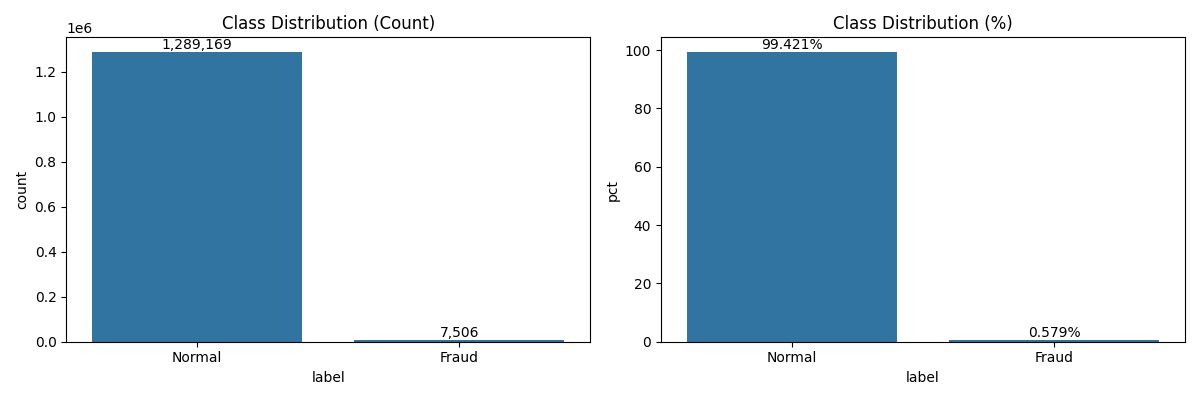
\includegraphics[width=0.9\linewidth]{Images/class_distribution.png}
    \caption{Class Distribution of Transactions (Count and Percentage)}
\end{figure}

\textbf{Analysis:}
\begin{itemize}
    \item The dataset is highly imbalanced, with normal transactions accounting for approximately 99.42\% of the data.
    \item Fraudulent transactions represent only about 0.58\%.
    \item This imbalance indicates that classification models may be biased toward the majority class.
    \item Special techniques such as resampling or class weighting are required.
\end{itemize}

% ---   

\subsubsection{Transaction Amount Distribution}

\begin{figure}[H]
    \centering
    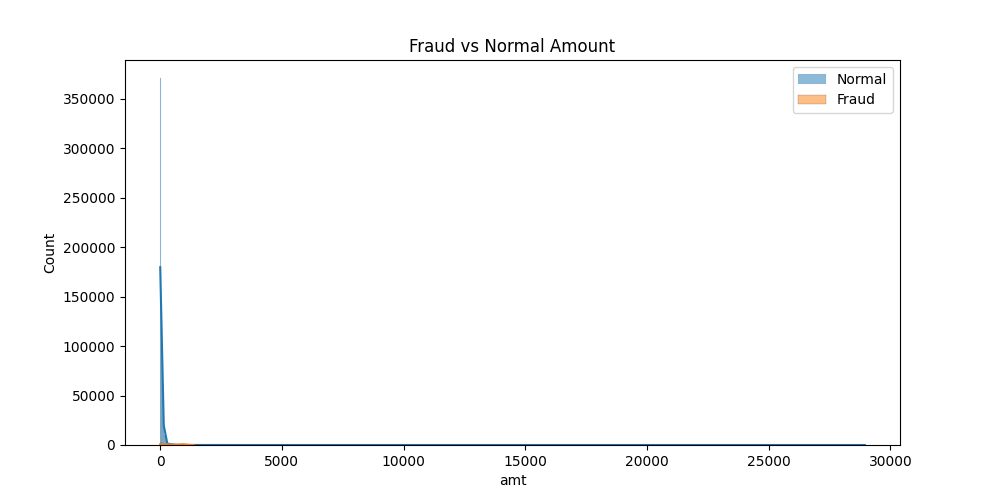
\includegraphics[width=0.9\linewidth]{Images/fraud_normal.png}
    \caption{Distribution of Transaction Amounts for Normal vs Fraudulent Transactions}
\end{figure}

\textbf{Analysis:}
\begin{itemize}
    \item The distribution of transaction amounts is highly skewed toward smaller values.
    \item Fraudulent transactions tend to have higher amounts compared to normal transactions.
    \item There is overlap between the two classes, indicating that transaction amount alone is insufficient for classification.
    \item The presence of extreme values suggests the existence of outliers.
\end{itemize}

% ---

\subsubsection{Time-Based Fraud Distribution}

\begin{figure}[H]
    \centering
    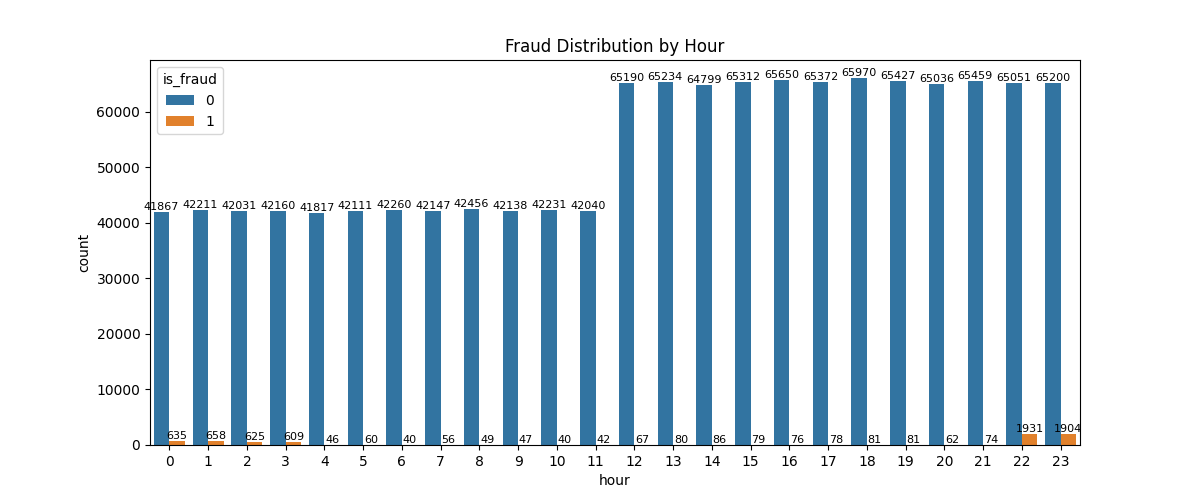
\includegraphics[width=0.9\linewidth]{Images/fraud_by_hour.png}
    \caption{Fraud Distribution by Hour of the Day}
\end{figure}

\textbf{Analysis:}
\begin{itemize}
    \item Transactions occur throughout all hours of the day.
    \item Fraudulent activities are present at every hour but remain relatively sparse.
    \item A slight increase in fraud can be observed during late hours.
    \item This suggests that temporal features may help improve fraud detection performance.
\end{itemize}

% ---

\subsubsection{Category-Based Fraud Rate}

\begin{figure}[H]
    \centering
    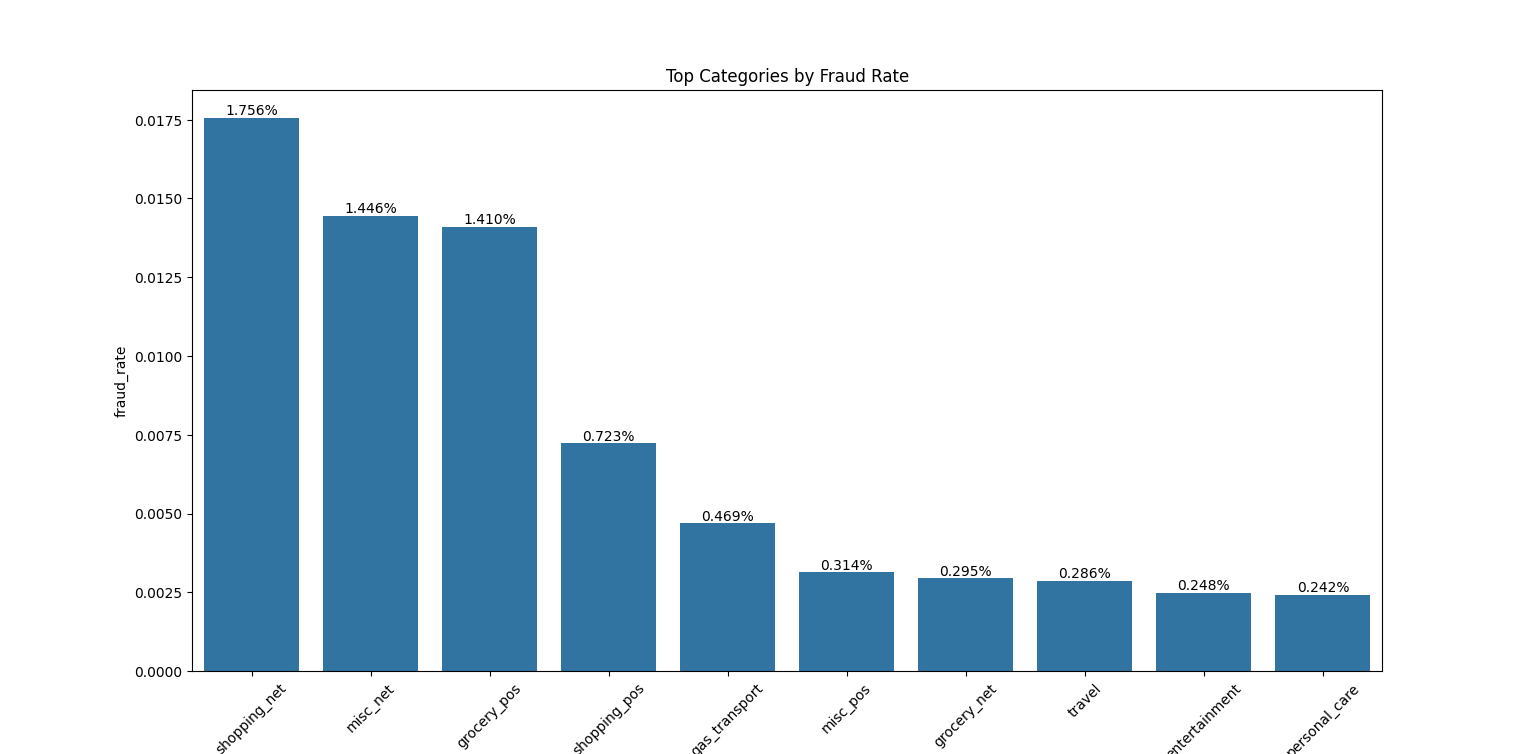
\includegraphics[width=0.9\linewidth]{Images/top_categories.png}
    \caption{Top Transaction Categories by Fraud Rate}
\end{figure}

\textbf{Analysis:}
\begin{itemize}
    \item Certain categories, particularly online-related categories (e.g., shopping\_net), exhibit higher fraud rates.
    \item Fraudulent activities are more prevalent in e-commerce transactions.
    \item This highlights the importance of the category feature in fraud detection.
\end{itemize}

% ---

\subsubsection{Correlation Matrix}

\begin{figure}[H]
    \centering
    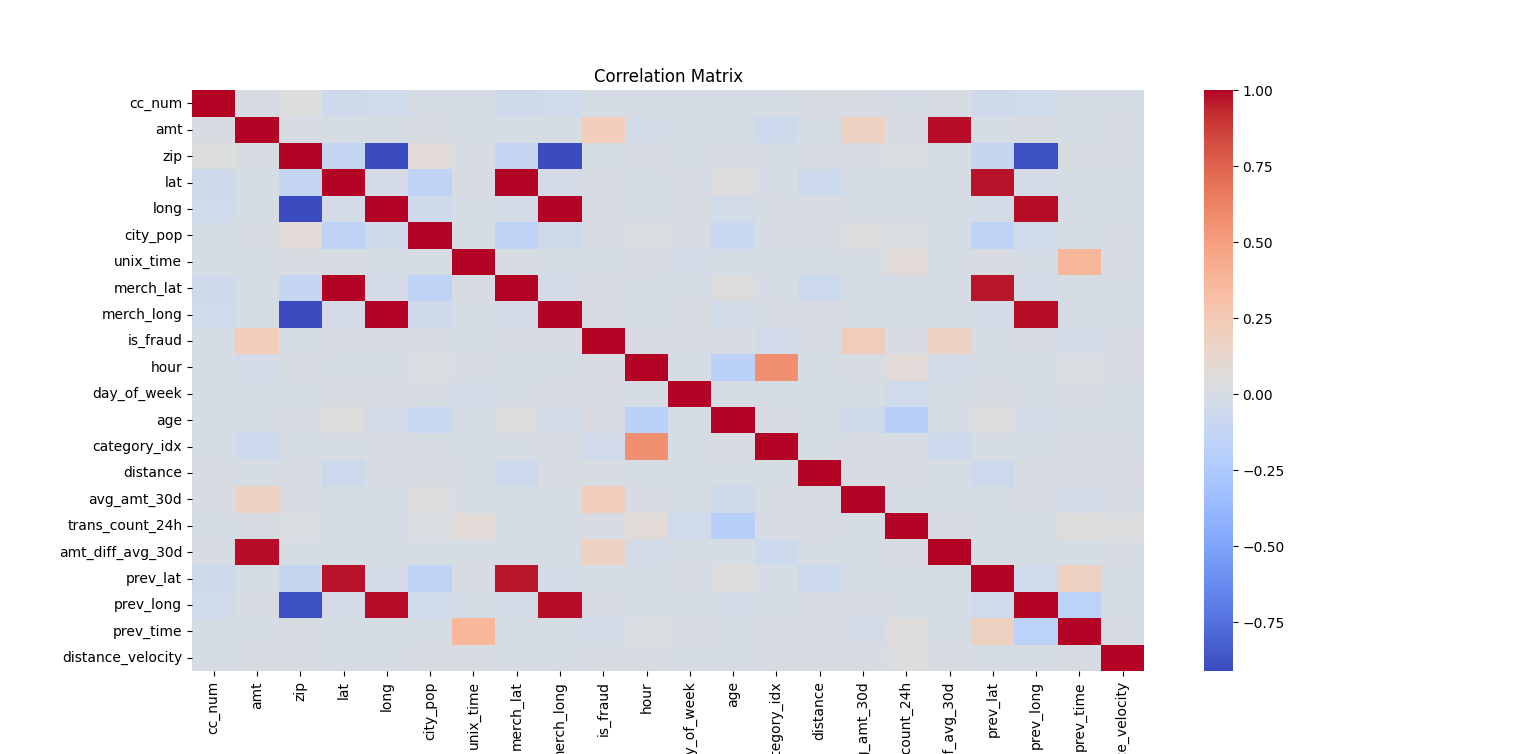
\includegraphics[width=0.9\linewidth]{Images/matrix.png}
    \caption{Correlation Matrix of Numerical Features}
\end{figure}

\textbf{Analysis:}
\begin{itemize}
    \item Strong correlations are observed between geographic features such as latitude and merchant latitude, as well as longitude and merchant longitude.
    \item Most features show weak correlation with the target variable.
    \item This indicates that fraud detection is a complex and non-linear problem.
    \item Advanced machine learning models are required to capture these relationships.
\end{itemize}

\subsubsection{Fraud Analysis by State}

To better understand geographical patterns in fraudulent transactions, the fraud rate was analyzed across all states (with at least 100 transactions to ensure statistical reliability).

\begin{figure}[H]
    \centering
    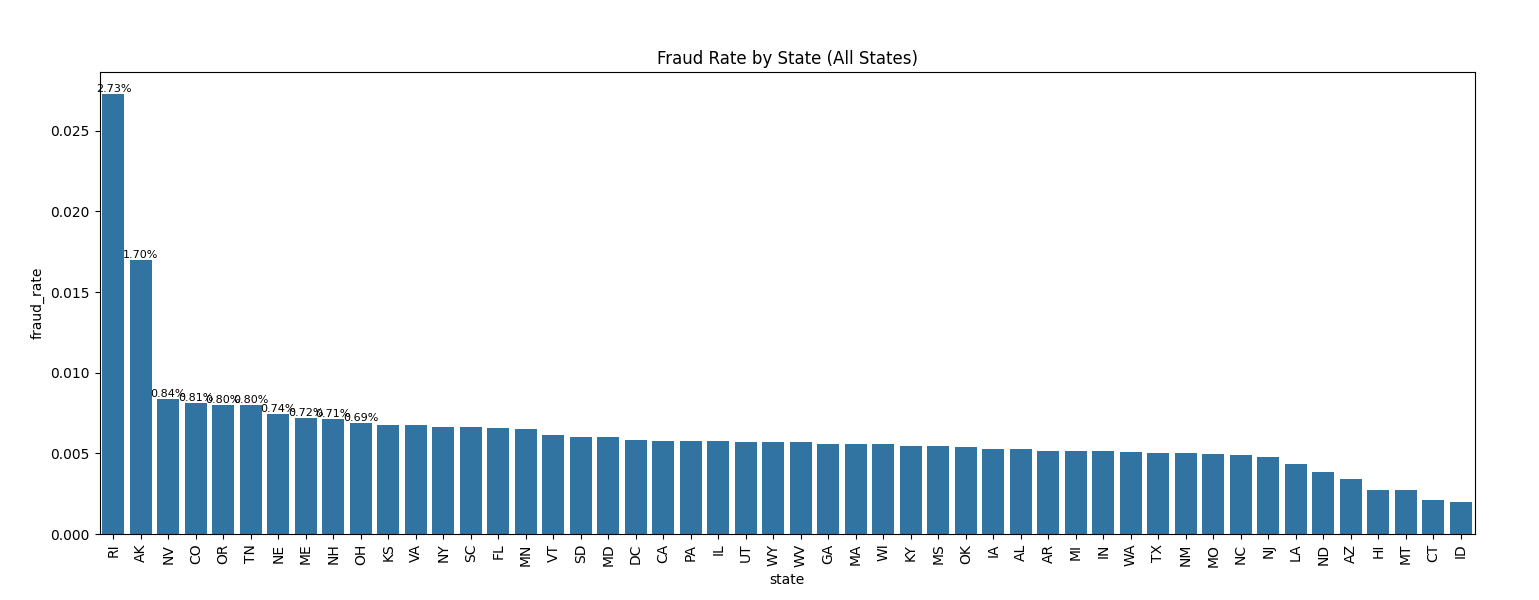
\includegraphics[width=0.9\linewidth]{Images/state.png}
    \caption{Fraud rate by state}
\end{figure}

\textbf{Key Observations:}
\begin{itemize}
    \item Fraud rates vary significantly across states, ranging from approximately \textbf{0.20\% to 2.73\%}.
    
    \item The state with the highest fraud rate is:
    \begin{itemize}
        \item \textbf{RI (Rhode Island)}: 2.73\% (15 fraud cases out of 550 transactions)
    \end{itemize}
    
    However, this state has a relatively small number of transactions, which may lead to higher variance and less reliable estimates.
    
    \item Other states with relatively high fraud rates include:
    \begin{itemize}
        \item AK (1.70\%)
        \item NV (0.84\%)
        \item CO (0.81\%)
        \item OR (0.80\%)
    \end{itemize}
    
    \item Most states have fraud rates clustered around \textbf{0.5\% to 0.7\%}, which is close to the overall dataset average (0.58\%).
    
    \item States with the lowest fraud rates include:
    \begin{itemize}
        \item ID (0.20\%)
        \item CT (0.21\%)
        \item MT (0.27\%)
        \item HI (0.27\%)
    \end{itemize}
    
    \item Large states with high transaction volumes such as:
    \begin{itemize}
        \item CA (0.58\%)
        \item TX (0.50\%)
        \item NY (0.66\%)
    \end{itemize}
    tend to have fraud rates close to the global average, suggesting more stable and representative behavior.
\end{itemize}

\textbf{Conclusion:}
\begin{itemize}
    \item Fraud behavior shows geographical variation, but extreme values often occur in states with low transaction counts.
    \item Location-based features (e.g., state) can contribute to fraud detection but should be combined with other features to avoid overfitting to small regions.
\end{itemize}

\subsubsection{Fraud Analysis by Gender}

Fraud distribution was also analyzed based on customer gender.
\begin{figure}[H]
    \centering
    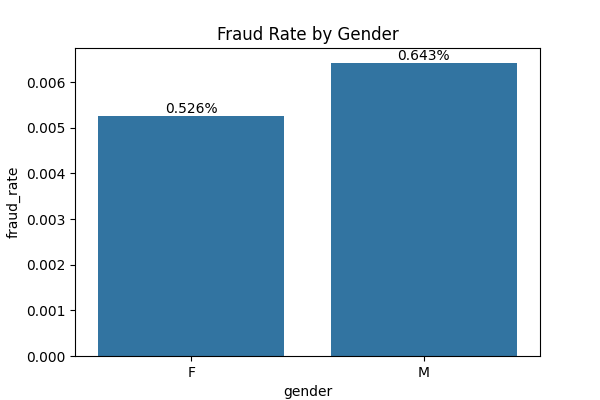
\includegraphics[width=0.9\linewidth]{Images/gender.png}
    \caption{Fraud rate by gender}
\end{figure}
\textbf{Statistics:}
\begin{itemize}
    \item Female:
    \begin{itemize}
        \item Fraud cases: 3,735
        \item Total transactions: 709,863
        \item Fraud rate: 0.526\%
    \end{itemize}
    
    \item Male:
    \begin{itemize}
        \item Fraud cases: 3,771
        \item Total transactions: 586,812
        \item Fraud rate: 0.643\%
    \end{itemize}
\end{itemize}

\textbf{Key Observations:}
\begin{itemize}
    \item Male customers have a slightly higher fraud rate than female customers:
    \begin{itemize}
        \item Difference: approximately \textbf{0.12\%}
    \end{itemize}
    
    \item Although the difference exists, it is relatively small, indicating that gender alone is not a strong predictor of fraud.
    
    \item Female customers have more total transactions, but a lower fraud rate, suggesting more stable transaction behavior overall.
\end{itemize}

\textbf{Conclusion:}
\begin{itemize}
    \item Gender has a minor impact on fraud likelihood.
    \item It can be used as a supporting feature in modeling but should not be relied upon as a primary indicator.
\end{itemize}